\documentclass[14pt,a4paper]{report}  %紙張設定
\usepackage{xeCJK}%中文字體模組
\setCJKmainfont{標楷體} %設定中文字體
%\setCJKmainfont{MoeStandardKai.ttf}
\newfontfamily\sectionef{Times New Roman}%設定英文字體
%\newfontfamily\sectionef{Nimbus Roman}
\usepackage{enumerate}
\usepackage{amsmath,amssymb}%數學公式、符號
\usepackage{amsfonts} %數學簍空的英文字
\usepackage{graphicx, subfigure}%圖形
\usepackage{fontawesome5} %引用icon
\usepackage{type1cm} %調整字體絕對大小
\usepackage{textpos} %設定文字絕對位置
\usepackage[top=2.5truecm,bottom=2.5truecm,
left=3truecm,right=2.5truecm]{geometry}
\usepackage{titlesec} %目錄標題設定模組
\usepackage{titletoc} %目錄內容設定模組
\usepackage{textcomp} %表格設定模組
\usepackage{multirow} %合併行
%\usepackage{multicol} %合併欄
\usepackage{CJK} %中文模組
\usepackage{CJKnumb} %中文數字模組
\usepackage{wallpaper} %浮水印
\usepackage{listings} %引用程式碼
\usepackage{hyperref} %引用url連結
\usepackage{setspace}
\usepackage{lscape}%設定橫式
\lstset{language=Python, %設定語言
		basicstyle=\fontsize{10pt}{2pt}\selectfont, %設定程式內文字體大小
		frame=lines,	%設定程式框架為線
}
%\usepackage{subcaption}%副圖標
\graphicspath{{./../images/}} %圖片預設讀取路徑
\usepackage{indentfirst} %設定開頭縮排模組
\renewcommand{\figurename}{\Large 圖.} %更改圖片標題名稱
\renewcommand{\tablename}{\Large 表.}
\renewcommand{\lstlistingname}{\Large 程式.} %設定程式標示名稱
\hoffset=-5mm %調整左右邊界
\voffset=-8mm %調整上下邊界
\setlength{\parindent}{3em}%設定首行行距縮排
\usepackage{appendix} %附錄
\usepackage{diagbox}%引用表格
\usepackage{multirow}%表格置中
%\usepackage{number line}
%=------------------更改標題內容----------------------=%
\titleformat{\chapter}[hang]{\center\sectionef\fontsize{20pt}{1pt}\bfseries}{\LARGE 第\CJKnumber{\thechapter}章}{1em}{}[]
\titleformat{\section}[hang]{\sectionef\fontsize{18pt}{2.5pt}\bfseries}{{\thesection}}{0.5em}{}[]
\titleformat{\subsection}[hang]{\sectionef\fontsize{18pt}{2.5pt}\bfseries}{{\thesubsection}}{1em}{}[]
%=------------------更改目錄內容-----------------------=%
\titlecontents{chapter}[11mm]{}{\sectionef\fontsize{18pt}{2.5pt}\bfseries\makebox[3.5em][l]
{第\CJKnumber{\thecontentslabel}章}}{}{\titlerule*[0.7pc]{.}\contentspage}
\titlecontents{section}[18mm]{}{\sectionef\LARGE\makebox[1.5em][l]
{\thecontentslabel}}{}{\titlerule*[0.7pc]{.}\contentspage}
\titlecontents{subsection}[4em]{}{\sectionef\Large\makebox[2.5em][l]{{\thecontentslabel}}}{}{\titlerule*[0.7pc]{.}\contentspage}
%=----------------------章節間距----------------------=%
\titlespacing*{\chapter} {0pt}{0pt}{18pt}
\titlespacing*{\section} {0pt}{12pt}{6pt}
\titlespacing*{\subsection} {0pt}{6pt}{6pt}
%=----------------------標題-------------------------=%             
\begin{document} %文件
\sectionef %設定英文字體啟用
\vspace{12em}
\begin{titlepage}%開頭
\begin{center}   %標題  
\makebox[1.5\width][s] %[s] 代表 Stretch the interword space in text across the entire width
{\fontsize{24pt}{2.5pt}國立虎尾科技大學}\\[18pt]
\makebox[1.5\width][s]
{\fontsize{24pt}{2.5pt}機械設計工程系}\\[18pt]
\sectionef\fontsize{24pt}{1em}\selectfont\textbf
{
\vspace{0.5em}
cd2023 2a3-pj3bg5分組報告}\\[18pt]
%設定文字盒子 [方框寬度的1.5倍寬][對其方式為文字平均分分布於方框中]\\距離下方18pt
\vspace{1em} %下移
\fontsize{30pt}{1pt}\selectfont\textbf{網際足球場景設計}\\
\vspace{1em}
\sectionef\fontsize{30pt}{1em}\selectfont\textbf
{
\vspace{0.5em}
Web-based Foosball Scene Design}
 \vspace{2em}
%=---------------------參與人員-----------------------=%  
\end{center}
\begin{flushleft}
\begin{LARGE}

\hspace{32mm}\makebox[5cm][s]
{指導教授:\quad 嚴\quad 家\quad 銘\quad 老\quad 師}\\[6pt]

\hspace{32mm}\makebox[5cm][s]
{班\qquad 級:\quad 四\quad 設\quad 二\quad 乙}\\[6pt]
\hspace{32mm}\makebox[5cm][s]
{學\qquad 生:\quad 梁\quad 琇\quad 婷\quad(41023202)}\\[6pt]
\hspace{32mm}\makebox[5cm][s]
{\hspace{36.5mm}張\quad 詠\quad 淇\quad(41023212)}\\[6pt]
\hspace{32mm}\makebox[5cm][s]
{\hspace{36.5mm}陳\quad 濬\quad 祺\quad(41023229)}\\[6pt]
\hspace{32mm}\makebox[5cm][s]
{\hspace{36.5mm}廖\quad 旭\quad 宏\quad(41023242)}\\[6pt]
\hspace{32mm}\makebox[5cm][s]
{\hspace{36.5mm}鄭\quad 煜\quad 橙\quad(41023252)}\\[6pt]
\hspace{32mm}\makebox[5cm][s]
{\hspace{36.5mm}吳\quad 圳\quad 吉\quad(40923115)}\\[6pt]
\hspace{32mm}\makebox[5cm][s]
{\hspace{36.5mm}林\quad 祐\quad 詮\quad(40923130)}\\[6pt]
\hspace{32mm}\makebox[5cm][s]
{\hspace{36.5mm}詹\quad 侑\quad 儒\quad(40923235)}\\[6pt]
%設定文字盒子[寬度為5cm][對其方式為文字平均分分布於方框中]空白距離{36.5mm}\空白1em
\end{LARGE}
\end{flushleft}
\vspace{6em}
\fontsize{18pt}{2pt}\selectfont\centerline{\makebox[\width][s]
{中華民國\hspace{3em} 
112 \quad 年\quad 6\quad 月}}
\end{titlepage}
\newpage
%=------------------------摘要-----------------------=%
\renewcommand{\baselinestretch}{1.5} %設定行距
\pagenumbering{roman} %設定頁數為羅馬數字
\clearpage  %設定頁數開始編譯
\sectionef
\addcontentsline{toc}{chapter}{摘~~~要} %將摘要加入目錄
\begin{center}
\LARGE\textbf{摘~~要}\\
\end{center}
\begin{flushleft}
\fontsize{14pt}{20pt}\sectionef\hspace{12pt}\quad 此專題的分組需要改用 Python 的 zmqRemoteAPI 來進行控制。需要完成以下任務:使用 zmqRemoteAPI 控制八台雙輪車在足球場中 對戰。此外,還需要設計一個能在雙方瀏覽器中進行計分的系統。每個分組完成後,需要將相關議題、設計操作系統置於各組網站,並完成線上簡報和分組 PDF 報告書。\\[12pt]

\fontsize{14pt}{20pt}\sectionef\hspace{12pt}\quad 關於 zmqRemoteAPI:zmqRemoteAPI 是一個用於 Python 和 CoppeliaSim 之間通訊的工 具。下面是使用 zmqRemoteAPI 相對於其他 Python 和 CoppeliaSim 通訊方法的一些優點和缺點: 
\begin{enumerate}
\item 優點:快速高效、使用方便、跨平台兼容性\\
\item 缺點:與傳統的 Python remoteAPI 相比沒有缺點。\\[12pt]
\end{enumerate}

\fontsize{14pt}{20pt}\sectionef\hspace{12pt}\quad 使用 zmq Remote API 可以在 Python 中編寫代碼來控制 CoppeliaSim 中的 Bubblerob 模型。並且可以使用 Python 程式碼控制 Bubblerob 的移動和行為,並觀察結果。zmq Remote API 提供了一種高效且跨平台的方式,使 Python 和 CoppeliaSim 之間可以進行快速的通訊和交互。這使得您可以通過編寫 Python 程式碼來操縱和控制 Bubblerob 模型,並進行各種控制實驗。
\end{flushleft}
\newpage
%=--------------------Abstract----------------------=%
\renewcommand{\baselinestretch}{1.5} %設定行距
\addcontentsline{toc}{chapter}{Abstract} %將摘要加入目錄
\begin{center}
\LARGE\textbf\sectionef{Abstract}\\
\begin{flushleft}
\fontsize{14pt}{16pt}\sectionef\hspace{12pt}\quad The group project requires a switch to Python's zmqRemoteAPI for control. The following tasks need to be accomplished: using zmqRemoteAPI to control eight two-wheeled vehicles for a soccer match on a field. Additionally, a scoring system needs to be designed that allows scoring in both teams' browsers. After each group completes their tasks, they are required to document relevant issues, design the operational system on their respective group websites, and finalize an online presentation and a group PDF report.\\[12pt]

\fontsize{14pt}{16pt}\sectionef\hspace{12pt}\quad Regarding zmqRemoteAPI: zmqRemoteAPI is a communication tool used between Python and CoppeliaSim. Here are some advantages and disadvantages of using zmqRemoteAPI compared to other Python and CoppeliaSim communication methods:\\
\begin{enumerate}
\item Advantages:\\

Fast and efficient、Ease of use、Cross-platform compatibility.\\
\item Disadvantages:\\

There are no specific disadvantages of zmqRemoteAPI compared to traditional Python remoteAPI.\\[12pt]
\end{enumerate}

\fontsize{14pt}{16pt}\sectionef\hspace{12pt}\quad Using the zmq Remote API, you can write code in Python to control the Bubblerob model in CoppeliaSim. With Python code, you can control the movement and behavior of Bubblerob and observe the results. The zmq Remote API provides an efficient and cross-platform method for fast communication and interaction between Python and CoppeliaSim. This allows you to manipulate and control the Bubblerob model by writing Python code and conduct various control experiments.
\end{flushleft}
\begin{center}
\fontsize{14pt}{16pt}\selectfont\sectionef Keyword:  nerual network、reinforcement learning、 CoppeliaSim、OpenAI Gym
\end{center}

\newpage
%=------------------------誌謝----------------------=%
\addcontentsline{toc}{chapter}{誌~~~謝}
\centerline\LARGE\textbf{誌~~謝}\\
\begin{flushleft}
\fontsize{14pt}{2.5pt}\hspace{12pt}\quad 在此鄭重感謝製作以及協助本分組報告完成的所有人員,首先向嚴家銘老師致謝,他們不辭辛勞解決我們的提問,甚至從來沒有不耐煩,總是貼心為我們找出最佳解答。再來是其他組的同學,提供我們解決問題的建議,最後是由本分組成員同心協力才得以完成本報告,特此感謝。 
\end{flushleft}
\newpage
%=------------------------目錄----------------------=%
\renewcommand{\contentsname}{\centerline{\fontsize{18pt}{\baselineskip}\selectfont\textbf{目\quad 錄}}}
\tableofcontents  %目錄產生
\newpage
%=------------------圖表目錄產生----------------------=%
\renewcommand{\listfigurename}{\centerline{\fontsize{18pt}{\baselineskip}\selectfont\textbf{圖\quad 目\quad 錄 }}}
\newcommand{\loflabel}{圖} %定義\loflabel 文字為圖
\renewcommand{\numberline}[1]{\loflabel~#1\hspace*{0.5em}}
\listoffigures
%\newcommand{\captioname}{圖}
\newpage
\renewcommand{\listtablename}{\centerline{\fontsize{18pt}{\baselineskip}\selectfont\textbf{表\quad 目\quad 錄 }}}
\newcommand{\lotlabel}{表} %定義\lotlabel 文字為表
\renewcommand{\numberline}[1]{\lotlabel~#1\hspace*{0.5em}}
\listoftables

\end{center}
%=-------------------------內容----------------------=%
\chapter{更新網站步驟}
\renewcommand{\baselinestretch}{10.0} %設定行距
\pagenumbering{arabic} %設定頁號阿拉伯數字
\setcounter{page}{1}  %設定頁數
\fontsize{14pt}{2.5pt}\sectionef
\section{詳細步驟說明}
機器學習與各領域結合的應用越來越廣泛,在機電系統採用強化學習是為了讓機電系統的控制達到最佳化。本專題以實體的冰球機,之機電系統作為訓練模型,將實體機器轉移到虛擬環境,進行模擬,為了找到適合的訓練參數,因此將模型簡化後再進行測試各種參數的優劣,透過不斷的訓練來得到一個優化過的對打系統。\\
\begin{itemize}
\item 個人的 fork 倉儲點選 sync fork 
\item 打開資料夾 
\item \texttt{點選 start\_ipv6.bat}
\item 輸入cd 資料夾名稱 並且git pull 
\item cms 
\item 貼上網址進行動態網頁編輯 
\item acp 
\item 點選個人 fork 倉儲 Open pull request 
\item 回到整組倉儲 merge pull request
\end{itemize}

\chapter{group}

\newpage

\chapter{會議記錄}
\section{5月23日會議紀錄}
討論事項: 討論機器人規格。首先繪製出各自的機器人。\\

\begin{figure}[hbt!]
\begin{center}
\label{523會議紀錄}
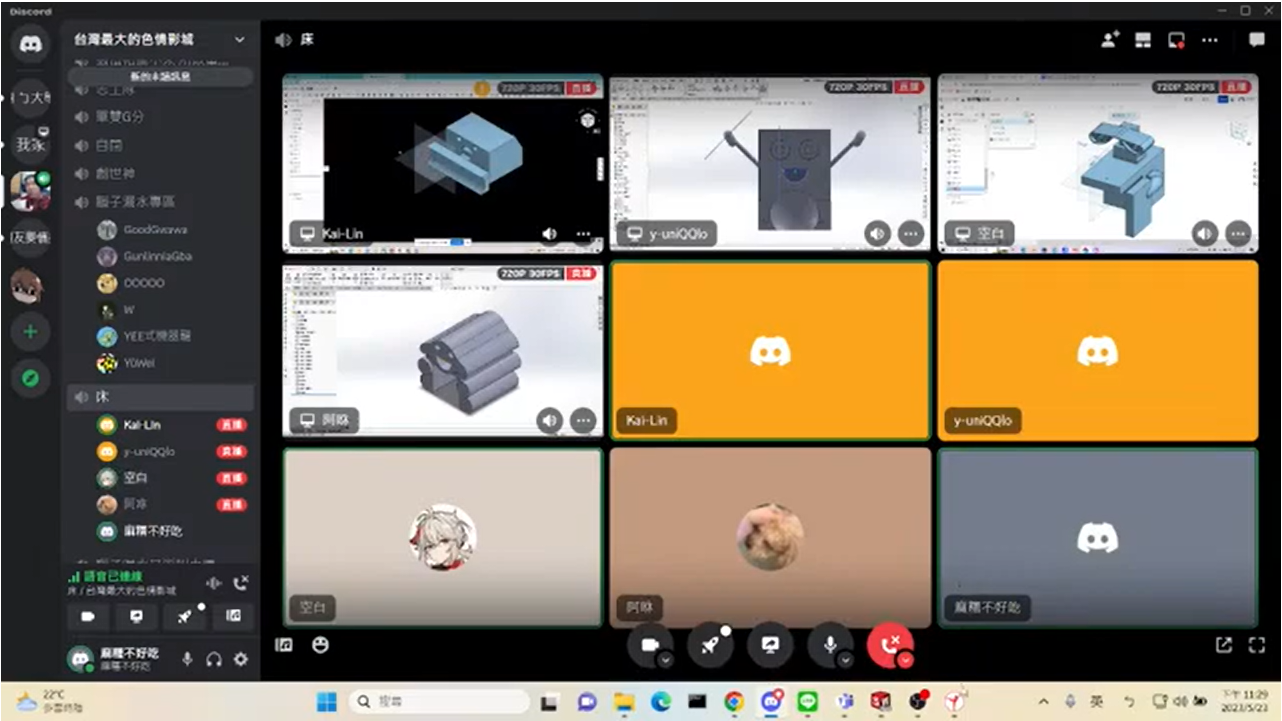
\includegraphics[width=12cm]{523開會紀錄}
\caption{\Large 523會議紀錄}
\end{center}
\end{figure}

\section{5月24日會議紀錄}
討論事項: 今日工作報告。\\

\begin{figure}[hbt!]
\begin{center}
\label{524會議紀錄}
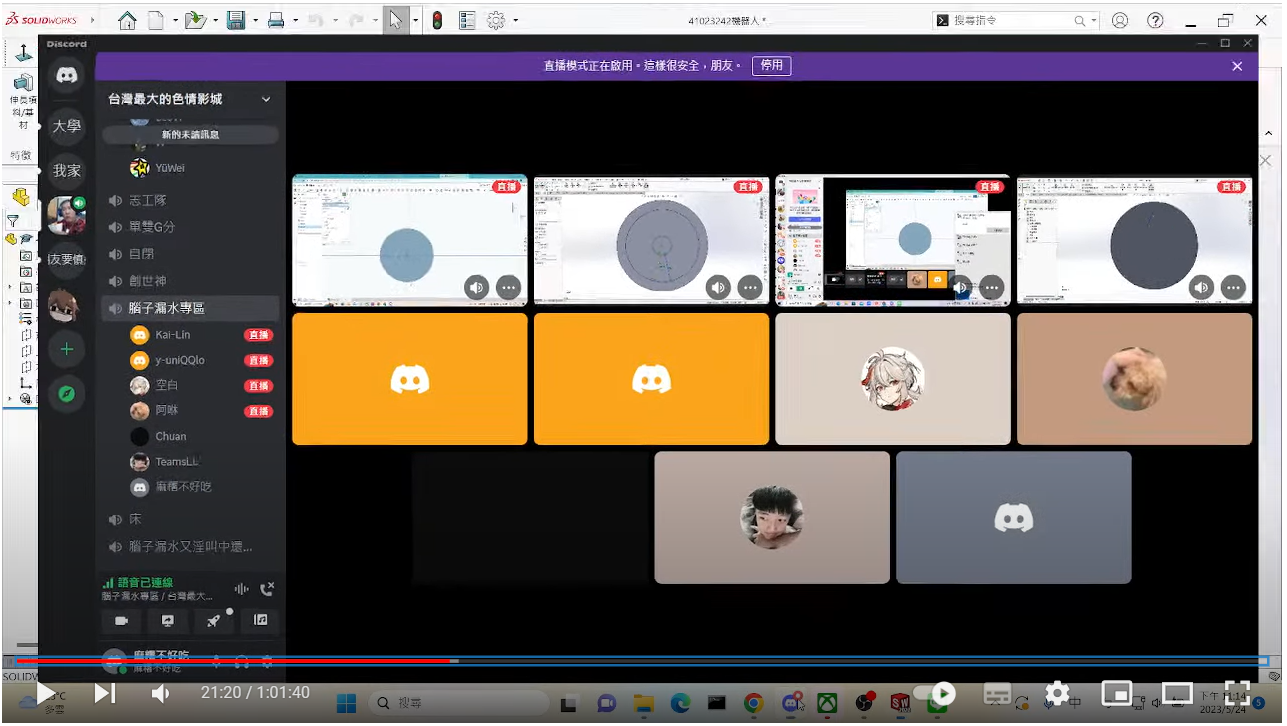
\includegraphics[width=12cm]{524會議紀錄}
\caption{\Large 524會議紀錄}
\end{center}
\end{figure}

41023242: 主持會議、上傳會議影片,組裝軸、把機器人匯入至CoppeliaSim嘗試動動看\

41023202: 繪製球員和球框場地\

41023212: 督導、協助\

41023229: 繪製計分裝置\

41023252: 督導、協助\

40923235: 繪製球員\

40923130: 程式修改\

40923115: 繪製球員\

40923235: 繪製球員\\

\section{5月31日會議紀錄}
討論事項: 把各自的機器人做修改並上傳,我們把場地跟球框重畫了,之前是場地球框分開畫,現在我們畫在一起這樣在協同的過程中比較方便進行,最後有讓我們的機器人裝上軸並試著走走看。\\

\begin{figure}[hbt!]
\begin{center}
\label{531會議紀錄}
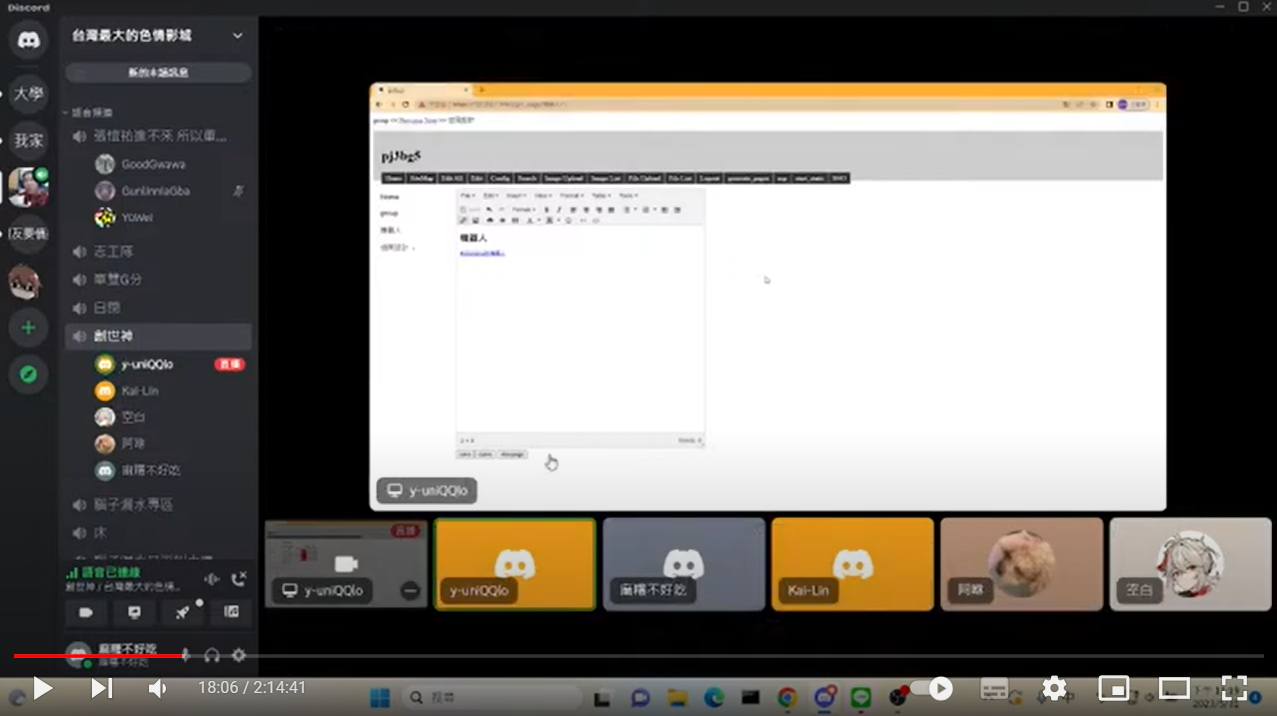
\includegraphics[width=12cm]{531會議紀錄}
\caption{\Large 531會議紀錄}
\end{center}
\end{figure}

\newpage

\chapter{分配工作}
%\renewcommand{\baselinestretch}{10.0} %設定行距
\begin{itemize}
\item 40923115:使用solidworks繪製機器人本體,按照規格所要求的畫,研究latex,轉成pdf,改良自己的機器人。
\item 40923130:繪製自己的機器人,更改joint與輪子名稱,寫wali程式碼,改良BubbleRob,寫BubbleRob程式碼,尋找與修改記分板程式碼。
\item 40923235:繪製自己的機器人,研究BubbleRob程式碼,撰寫latex、製作報告,並修正latex中遇到的錯誤。
\item 41023202:詢問許多同學步驟,首先先製作足球機器人。我是先用solidworks畫出機器人的本體,按照規格所要求的畫。之後再把檔案存成stl檔。接著畫出輪子(含輪框)、軸各為一份檔案。也是存成stl檔案。接著再畫出場地,按照尺寸設計以及需求,也是存成stl檔案。 
\item 41023212:負責畫出自己的機器人,並嘗試帶入計分器的程式,與別組已完成的同學討論,新增機器人背號。 
\item 41023229:負責畫機器人和裝機器人的軸作動跟畫記分板,組裝記分板和製作分組報告。
\item 41023242:負責主持會議、錄製影片、交代任務,尋找可能會發生哪些問題並盡快提早解決,畫機器人、畫記分板、組裝軸。
\item 41023252:負責畫出自己的機器人,將機器人裝上轉軸作動,解決cmd及網站倉儲問題,修改、測試記分板程式問題。
\end{itemize}
\newpage

\chapter{場景佈置}
\section{機器人}
\begin{figure}[hbt!]
\begin{center}
\label{各自機器人圖}
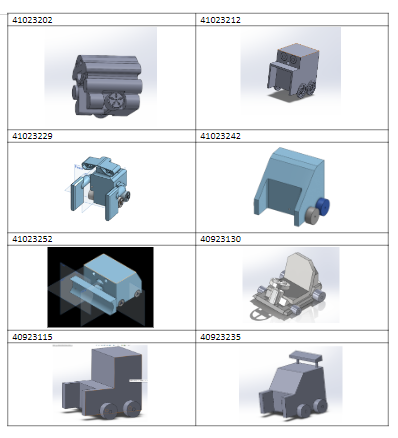
\includegraphics[width=\textwidth]{各自機器人圖}
\caption{\Large 機器人繪製}
\end{center}
\end{figure}

\section{記分板}
\begin{figure}[hbt!]
\begin{center}
\label{記分板}
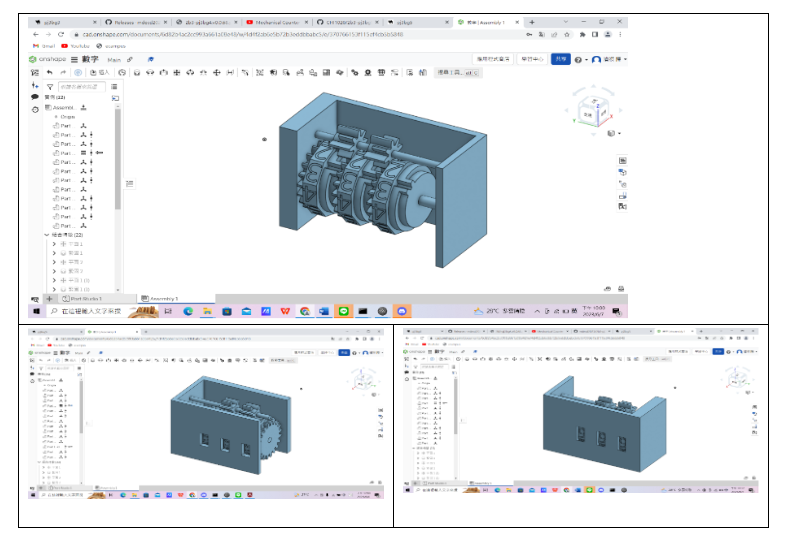
\includegraphics[width=\textwidth]{記分板}
\caption{\Large 記分板繪製}
\end{center}
\end{figure}

\chapter{Python程式碼}
\section{Wali}
\begin{figure}[!ht]
\centering
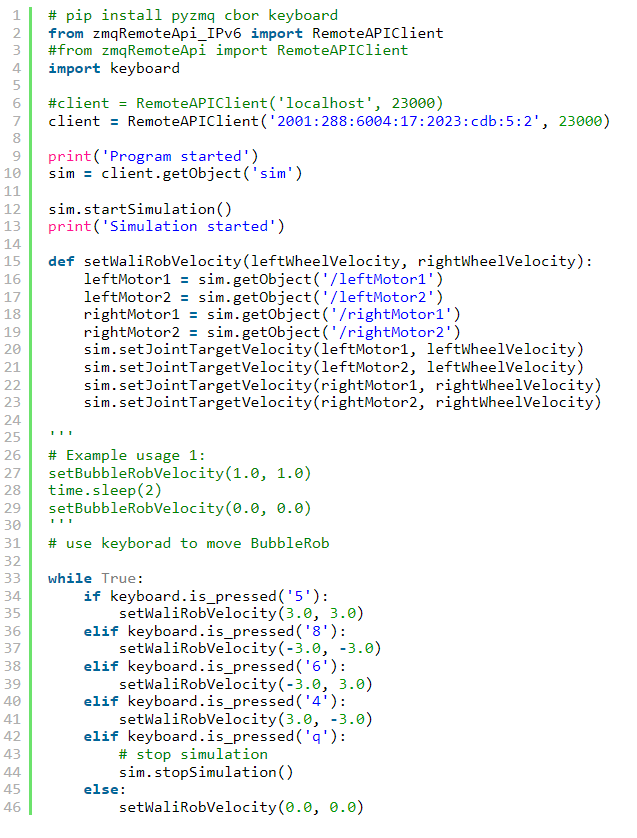
\includegraphics[width=\textwidth]{wali程式碼}
\caption{\Large wali程式碼}
\label{wali程式碼}
\end{figure}
\newpage

\section{4輪BubbleRob}
因為發現原有Wali機器人結構太複雜,放8隻機器人會導致操控上很延遲,所以將4隻改成PJ1和PJ2的BubbleRob改良成4個輪子,以下為程式碼。\\

\begin{figure}[!ht]
\centering
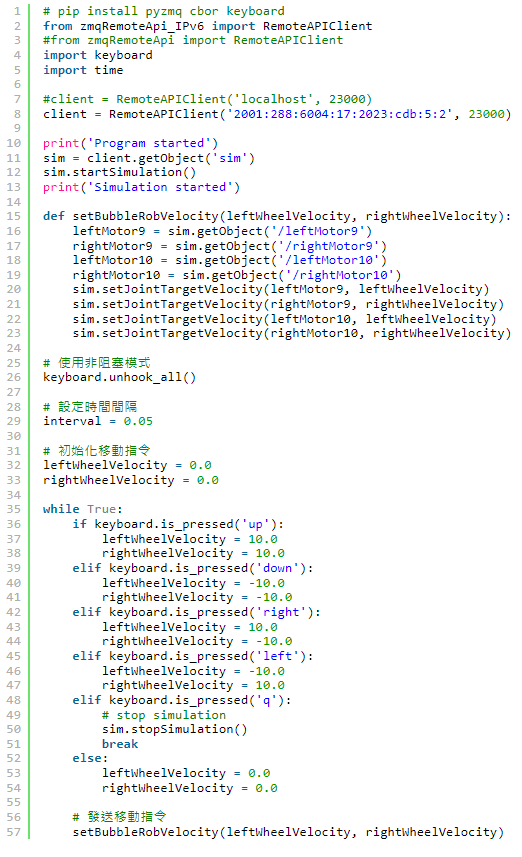
\includegraphics[width=\textwidth]{4輪BubbleRob程式碼}
\caption{\Large 4輪BubbleRob程式碼}
\label{4輪BubbleRob程式碼}
\end{figure}
\newpage

\section{記分板}
\begin{figure}[!ht]
\centering
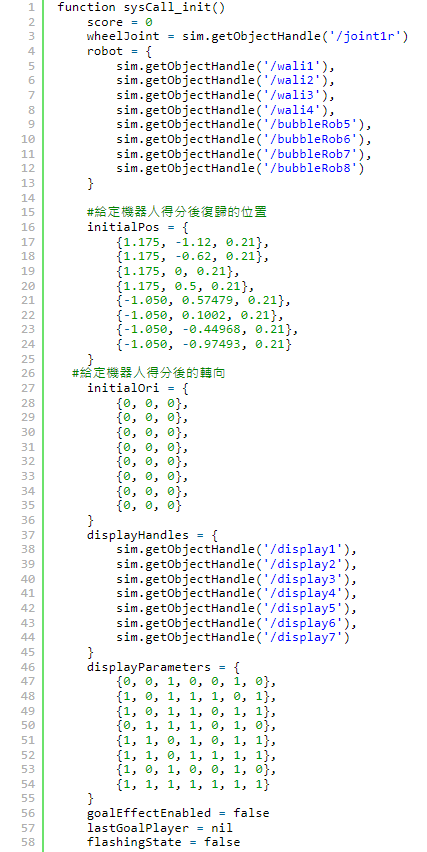
\includegraphics[width=\textwidth]{記分板程式碼前半}
\caption{\Large 記分板程式碼前半}
\label{4輪BubbleRob程式碼}
\end{figure}
\begin{figure}[!ht]
\centering
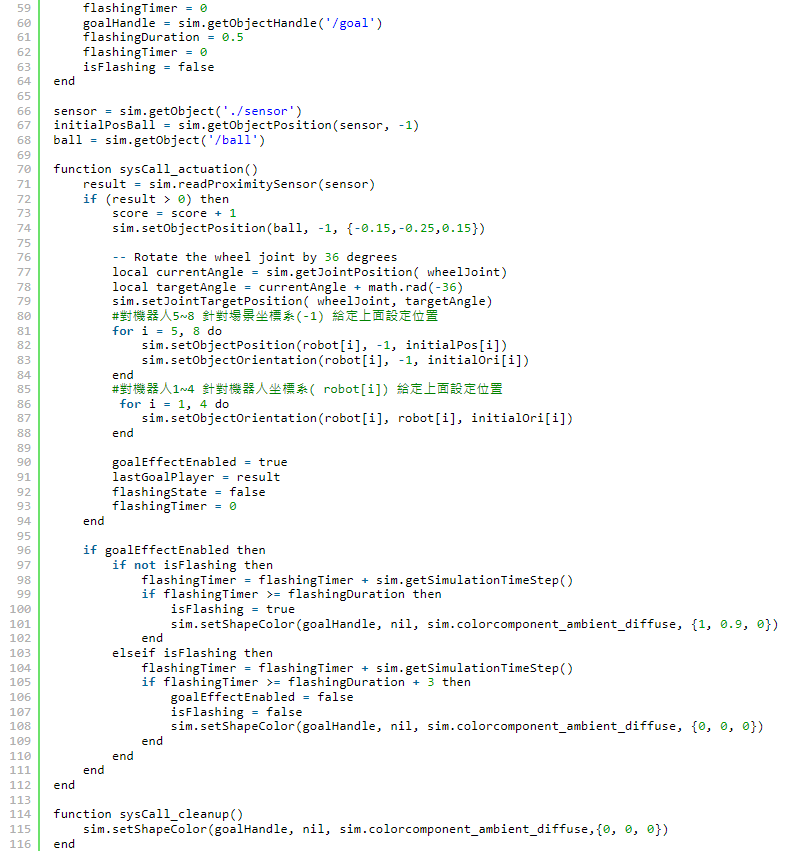
\includegraphics[width=\textwidth]{記分板程式碼後半}
\caption{\Large 記分板程式碼後半}
\label{4輪BubbleRob程式碼}
\end{figure}

\newpage

\chapter{Latex錯誤修正}
在製作latex報告中,經常會出現錯誤,在不懂錯誤的情況下,詢問chatGPT尋求解答\\

\begin{figure}[ht]
  \begin{minipage}{0.5\textwidth}
    \centering
    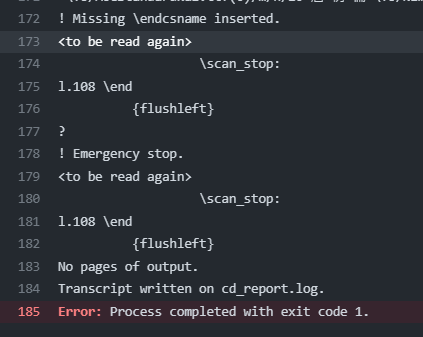
\includegraphics[width=\textwidth]{beginend錯誤}
    \caption{latex錯誤1}
  \end{minipage}%
  \begin{minipage}{0.5\textwidth}
    \centering
    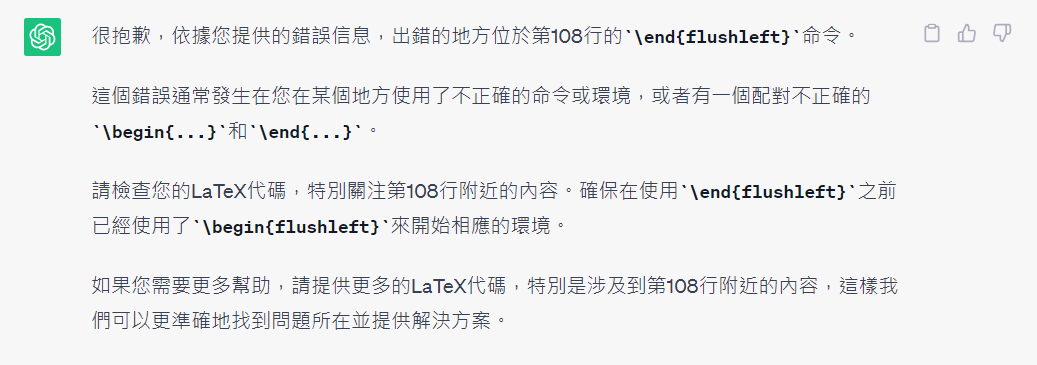
\includegraphics[width=\textwidth]{beginend錯誤解答}
    \caption{latex錯誤回答1}
  \end{minipage}
\end{figure}

此情況可能為begin跟end數量不對等造成的錯誤。\\

\begin{figure}[ht]
  \begin{minipage}{0.5\textwidth}
    \centering
    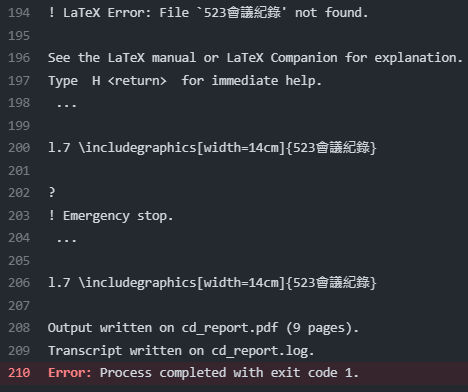
\includegraphics[width=\textwidth]{圖片名打錯}
    \caption{latex錯誤2}
  \end{minipage}%
  \begin{minipage}{0.5\textwidth}
    \centering
    
\includegraphics[width=\textwidth]{圖片名打錯解答}
    \caption{latex錯誤回答2}
  \end{minipage}
\end{figure}

在[width]後面接的是image裡面的圖檔名稱,要在目錄中顯示的名稱要打在caption後面。\\

\begin{figure}[ht]
  \begin{minipage}{0.5\textwidth}
    \centering
    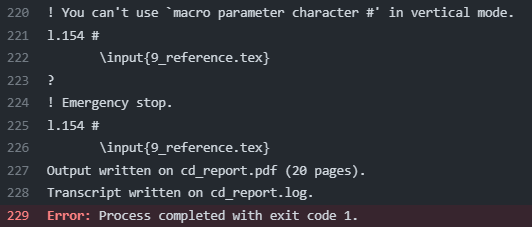
\includegraphics[width=\textwidth]{符號打錯}
    \caption{latex錯誤3}
  \end{minipage}%
  \begin{minipage}{0.5\textwidth}
    \centering
    
\includegraphics[width=\textwidth]{符號打錯解答}
    \caption{latex錯誤回答3}
  \end{minipage}
\end{figure}

在latex程式碼中,想要屏蔽不想要出現的內容,不能打\#,要在該段最前面輸入\%。\\

\begin{figure}[ht]
  \begin{minipage}{0.5\textwidth}
    \centering
    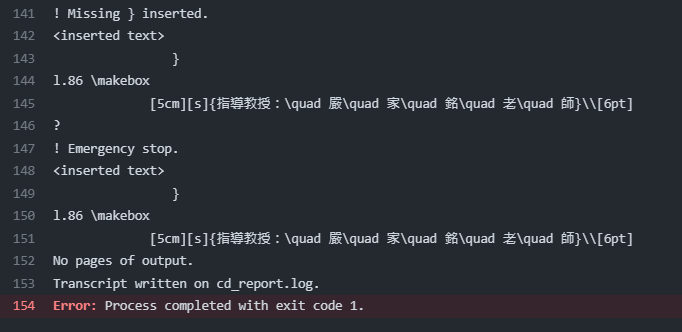
\includegraphics[width=\textwidth]{缺少符號}
    \caption{latex錯誤4}
  \end{minipage}%
  \begin{minipage}{0.5\textwidth}
    \centering
    
\includegraphics[width=\textwidth]{缺少符號解答}
    \caption{latex錯誤回答4}
  \end{minipage}
\end{figure}

要注意是否都有輸入正確的符號,括號要對稱。\\

\begin{figure}[ht]
  \begin{minipage}{0.5\textwidth}
    \centering
    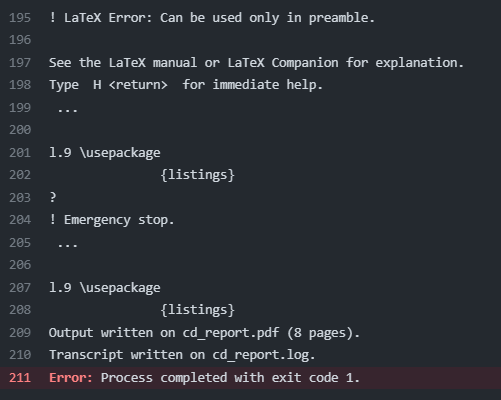
\includegraphics[width=\textwidth]{設定錯誤}
    \caption{latex錯誤5}
  \end{minipage}%
  \begin{minipage}{0.5\textwidth}
    \centering
    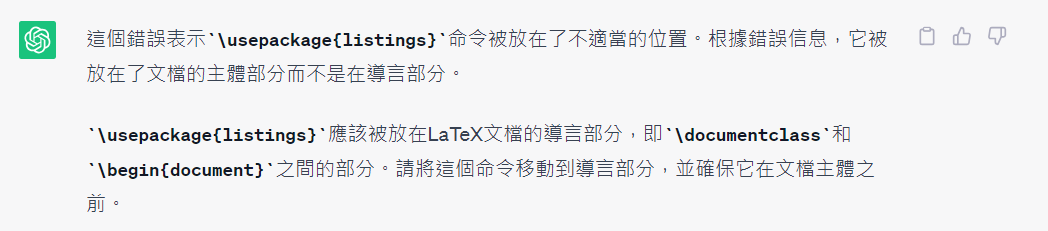
\includegraphics[width=\textwidth]{設定錯誤解答}
    \caption{latex錯誤回答5}
  \end{minipage}
\end{figure}

設定文章內容的條件應該要放在最前頁,不能放在篇章中。
\newpage

\chapter{latex與word比較}
LaTex 為一種程式語言,支援標準庫 (Standard Libraries) 和外部程式庫 (External Libraries),不過與一般程式語言不同的是,它可以直接表述 Tex 排版結構,類似於 PHP 之於 HTML 的概念。但是直接撰寫 LaTex 仍較複雜,因此可以藉由 Markdown 這種輕量的標註式語言先行完成文章,再交由 LaTex 排版。\\

此報告採用編輯軟體為LaTeX,綜合對比Word編輯方法,LaTeX較為精準正確、更改、製作公式等,以便符合規範、製作。
 \begin{table}[htbp] %htbp代表表格浮動位置
			\centering%表格居中
			\caption{文字編輯軟體比較表}%表:標題
			\large%字體大小
			\label{tab_文字編輯軟體比較表:scale}
			\begin{tabular}{|c|c|c|c|c|c|c|}
			\hline
			\diagbox[width=5em]& 相容性 & 直觀性 & 文件排版 & 數學公式 & 微調細部\\ 
			\hline
			LaTeX 		&$\surd$&		&$\surd$&$\surd$&$\surd$\\
			\hline
			Word	 	&		&$\surd$&		&		&$\surd$\\
			\hline
			
			\end{tabular}
		\end{table}	
\end{appendix}
\begin{itemize} 
\item 特點:
\end{itemize}
\begin{enumerate}
\item 相容性:以Word為例會有版本差異,使用較高版本編輯的文件可能無法以較低的版本開啟,且不同作業系統也有些許差異;相比LaTeX可以利用不同編譯器進行編譯,且為免費軟體也可移植至可攜系統內,可以搭配Github協同編譯。
\item 文件排版:許多規範都會要求使用特定版型,使用文字編譯環境較能準確符合規定之版型,且能夠大範圍的自定義排定所需格式,並能不受之後更改而整體格式變形。
\item 數學公式呈現:LaTex可以直接利用本身多元的模組套件加入、編輯數學公式,在數學推導過程能夠快速的輸入自己需要的內容即可。
\item 細部調整:在大型論文、報告中有多項文字、圖片、表格,需要調整細部時,要在好幾頁中找尋,而LaTeX可以分段章節進行編譯,再進行合併處理大章節。
\end{enumerate}
\newpage


%\newpage
%\begin{landscape}  %橫式環境
%\begin{center}
%\fontsize{0.001pt}{1pt}\selectfont .
%\vspace{70mm}
%\rotatebox[origin=cc]{90}{\LARGE 【14】}\rotatebox[origin=cc]%{180}{\LARGE 1-2-APP-8765} %旋轉
%\end{center}
%\end{landscape}

\end{document}
